\graphicspath{{./Wstep/images}}

\chapter{Wstęp}

Placeholder.

\section{Grawitropizm}

Placeholder aż znajdę sensowną literaturę.

\section{Symulatory mikrograwitacji}

Istnieje wiele sposobów imitacji środowiska kosmiczego w warunkach ziemskich. Część z rozwiązań jest uniwersalna względem testowanych obiektów, niektóre zaś są w stanie symulować owe warunki tylko dla wąskiego rodzaju obiektów badawczych. Poniżej opisane zostało kilka popularnych typów takich symulatorów.

\subsection{Lot paraboliczny}

Stan nieważkości w przypadku tego symulatora generowany jest przez lot samolotu po odpowiedniej trajektorii. Przystosowany do tego samolot wznosi się oraz spada pod kątem 45$^\circ$. Gdy pojazd znajduje się na szczycie swojej trajektorii, cała zawartość samolotu doświadcza stanu nieważkości na czas około 20 sekund \cite{bib:lot_paraboliczny}. 

\begin{figure}[h]
	
	\centering
	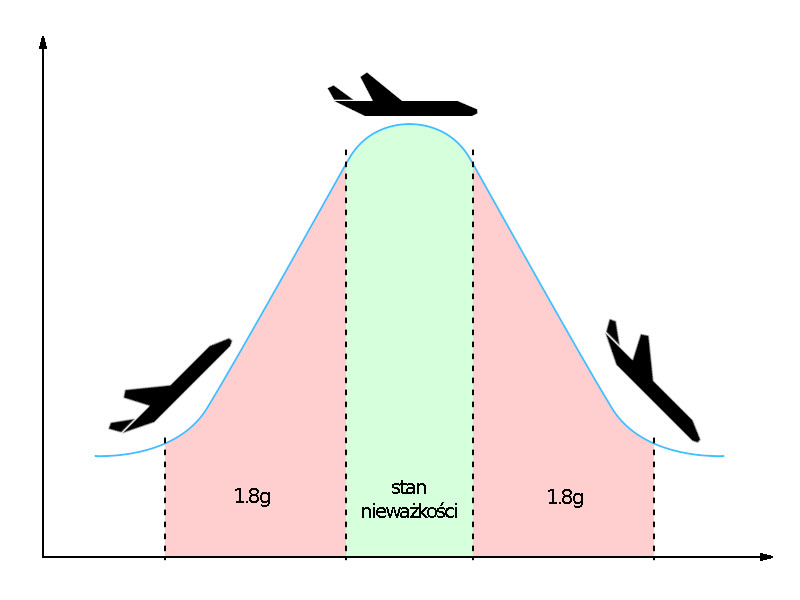
\includegraphics[scale=0.6]{lot_para_sch.jpg}
	\caption{Schemat trajektorii podczas lotu parabolicznego.}
	\label{Lot paraboliczny}
	
\end{figure}

Metoda ta jest bardzo przydatna ze względu na możliwość poddania względnie dużych przedmiotów na warunki mikrograwitacji. Obecnie jest to jedyna metoda umożliwiająca wystawienie astronautów na takie warunki, przed wysłaniem ich na Międzynarodową Stację Kosmiczną (ISS)\cite{bib:lot_paraboliczny}. Samolot może również poruszać się po łuku, symulując w ten sposób środowisko o obniżonej, niezerowej grawitacji. Z tego typu symulatorów korzysta się również w początkowych etapach badań, przed decyzją o wysłanie obiektów badawczych w kosmos. Pozwala to zebrać użyteczne dane wstępne jak i zmodyfikować parametry eksperymentu docelowo przeprowadzanego w kosmosie. Wadą tego rozwiązania jest przede wszystkim krótki okres w którym ładunek doświadcza stanu nieważkości.

\subsection{Systemy LSMM}

LSMM jest nazwą obejmującą szeroką gamę symulatorów używanych w przypadku próbek biologicznych. Ta grupa urządzeń symuluje pewne konkretne cechy środowiska kosmicznego takie jak brak sedymentacji, niskie naprężenia ścinające w płynach oraz niewielkie turbulencje\cite{bib:lsmm1}. Zwykle urządzenia tego typu wykorzystują rotację całej próbki aby osiągnąć wspomniane wcześniej cechy środowiska. Pierwsze bioreaktory rozwijane były przez Centrum Lotów Kosmicznych im. Lyndona B. Johnsona \cite{bib:lsmm1}, które służyły do badania rozwoju mikroorganizmów w warunkach mikrograwitacji. Tego typu urządzenia są zwykle kategoryzowane jako RWV, które następnie obejmuje wiele różnych konfiguracji takich jak HARV, STLV, RWPV. W celach badań roślin, ludzkich komórek lub tkanek wykorzystuje się urządzenia nazywane klinostatami, które również należą do grupy systemów LSMM natomiast znacznie różnią się konstrukcją. Wariacją klinostatów są maszyny RPM. Tematyka tej pracy jest ściśle związana z klinostatami, a więc zostaną one omówione szczegółowo w dalszej części tego rozdziału.

\subsection{Lewitacja diamagnetyczna}

Kolejną metodą wykluczenia skutków oddziaływania siły grawitacji z próbką jest wykorzystanie interakcji diamagnetycznej. Diamagnetyzm jest fundamentalną cechą materii, powodowaną ruchem elektronów w atomach\cite{bib:kittel}. Zjawisko to można wykorzystać do lewitacji każdej substancji, wymagane jest jedynie odpowiednio silne zewnętrzne pole magnetyczne. Z uwagi na to iż diamagnetyzm jest oddziaływaniem bardzo słabym, stosowane są pola magnetyczne o indukcji rzędu $B=16.5 T$. Należy zaznaczyć iż aby osiągnąć stan lewitacji konieczne jest uzyskanie wysokiego przestrzennego gradientu pola magnetycznego, pole jednorodne nie będzie skutkować pojawieniem się sił związanych z diamagnetyzmem. Tego typu lewitacja została wykorzystana w badaniach nad rozwojem oraz ekspresją genów w muszkach owocowych (\ang{Drosophila melanogaster}) w warunkach mikrograwitacji\cite{bib:lewitacja}.

\subsection{Maszyny spadku swobodnego (FFM)}

Pierwsze maszyny spadku swobodnego zostały wynalezione jako alternatywa dla już wtedy istniejących klinostatów dwuwymiarowych. Zasada działania tych urządzeń opiera się na grawitacyjnym spadku swobodnym próbki przymocowanej do wózka ślizgającego się wzdłuż pionowych szyn o długości \SI{1}{m}. Gdy próbka opada na dół urządzenia, podmuch sprężonego powietrza o ciśnieniu \SI{8}{bar} odbija próbkę z powrotem na górę szyny i cykl się powtarza. Próbka podczas powrotu na górę szyny doświadcza bardzo wysokiego przyspieszenia przez krótki czas, który jest na tyle krótki, aby był pomijalny z punktu widzenia badanego obiektu.

\section{Klinostaty}


\section{Zasada działania klinostatu}

\section{Rodzaje klinostatów}

\section{Obecne rozwiązania}